\chapter{Organisation et gestion de données}
{https://sacado.xyz/qcm/parcours_show_course/0/117141}
{
\begin{CpsCol}
 \textbf{Les savoir-faire du parcours}
 \begin{itemize}
 \item Savoir lire et compléter des données dans un tableau.
 \item Savoir lire et construire un diagramme en bâtons.
 \item Savoir utiliser et construire un diagramme circulaire.
 \item Savoir utiliser et construire un diagramme cartésien.
 \end{itemize}
\end{CpsCol}

\textbf{qrcode vers le parcours diagnostic}

}

\begin{pageCours} 

\section{Tableaux}

\begin{DefT}{Tableau simple}

Les \textbf{tableaux}\index{Tableau} permettent d'organiser et de regrouper des données pour les lire plus facilement.
\begin{itemize}
\item On utilise un tableau à \textbf{une seule entrée}\index{Simple|Tableau} pour organiser des données selon \textbf{un seul critère}.
\item On utilise un tableau à \textbf{double entrée}\index{A double entrée|Tableau} pour organiser des données selon \textbf{deux critères}, l'un qui est lu en ligne et l'autre en colonne.
\end{itemize}

\end{DefT}


\begin{ExT}{Tableau simple}

On a mesuré la taille d'une pousse de bambou lors des 6 premiers mois après sa plantation.
 \begin{center}
 \begin{tabular}{|c|c|c|c|c|c|c|} 
  \hline
  Mois & Novembre & Décembre & Janvier  & Février & Mars & Avril \\
  \hline
  Taille (cm) & \textcolor{sacado_green}{$70$} & $100$ & $127$ & \textcolor{sacado_violet}{$150$} & $180$ & \textcolor{sacado_orange}{$212$}  \\
  \hline
 \end{tabular}
 \end{center}

La pousse de bambou mesurent \textcolor{sacado_green}{$70$} cm lors de sa plantation en décembre. Au mois de février, elle mesure \textcolor{sacado_violet}{$150$} cm et \textcolor{sacado_orange}{$212$} cm en avril .
\end{ExT}


\begin{ExT}{Tableau à double entrée}

	Voici les résultats d'une enquête réalisée dans un collège sur le moyen de locomotion des élèves.

 \begin{center}
 \begin{tabular}{|c|c|c|c|c|c|c|} \hline
  Locomotion & A pied & Voiture & Bus &  Vélo & Autres & Total \\  \hline
  Garçons & $92$ & $36$ & \textcolor{sacado_orange}{$118$}& $54$ & $25$ & \textcolor{sacado_blue}{$325$} \\\hline
  Filles &  $94$ & $40$ & $197$ & \textcolor{sacado_violet}{$40$}  & $33$ & \textcolor{sacado_green}{$404$} \\\hline
  Total & \textcolor{sacado_gray}{$186$} & $76$ & $315$& \textcolor{sacado_red}{$94$} & $58$ & $729$ \\ \hline
 \end{tabular}
 \end{center}
 
\begin{itemize}
 \item Dans ce collège, il y a \textcolor{sacado_green}{$404$} filles et \textcolor{sacado_blue}{$325$} garçons.
 \item \textcolor{sacado_gray}{$186$} élèves viennent à pied et \textcolor{sacado_red}{$94$} en vélo.
 \item \textcolor{sacado_violet}{$40$} filles viennent en vélo et \textcolor{sacado_orange}{$118$} garçons viennent en bus.
\end{itemize}

\end{ExT}

\end{pageCours}




\begin{pageAD} 

\Sf{Savoir lire des données dans un tableau à double entrée}

\ExoCad{Chercher. Communiquer. }

Voici les résultats d'une enquête réalisée dans un collège.

 \begin{center}
 \begin{tabular}{|c|c|c|c|}\hline 
  & Demi-pensionnaires & Externes & Total \\\hline 
  Garçons & $145$ & $173$ & $318$ \\\hline
  Filles & $70$ & $289$ & $359$ \\\hline
  Total & $215$ & $462$ & $677$ \\\hline 
 \end{tabular}
 \end{center}
 
 \begin{enumerate}
 \item Quelles sont les deux entrées de ce tableau ? \point{2}
 \item Combien y a-t-il de garçons ? \point{1}
 \item Combien y a-t-il d'élèves externes ? \point{1}
 \item Combien d'élèves sont des filles demi-pensionnaires ? \point{1} 
 \item Que représente $173$ ? \point{1} 
\end{enumerate}

\Sf{Savoir compléter un tableau}

\ExoCad{Représenter.}

Le centre météorologique a enregistré les températures moyenne sur les 4 premiers mois de l'année : 15°C en avril, 7°C en janvier, 12°C en mars et 9°C en février. Complète le tableau suivant.

 \begin{center}
 \begin{tabular}{|c|c|c|c|c|}\hline 
  Mois & Janvier & Février & Mars & Avril \\\hline 
  Température ($\ldots$)& $\ldots$ & $\ldots$ & $\ldots$ & $\ldots$ \\\hline
 \end{tabular}
 \end{center}


\ExoCad{Représenter.}

Au championnat du monde de judo 2023, le japon a obtenu 5 médailles d'or, 2 d'argent et 4 de bronze. La France a glané 2 médailles d'or, 3 d'argent et 2 de bronze. Complète le tableau suivant.

 \begin{center}
 \begin{tabular}{|c|c|c|c|c|}\hline 
  Pays $\setminus$ médailles& Or & Argent & Bronze & Total\\\hline 
  Japon & $\ldots$ & $\ldots$ & $\ldots$ & $\ldots$ \\\hline
  France & $\ldots$ & $\ldots$ & $\ldots$& $\ldots$  \\\hline
 \end{tabular}
 \end{center}


\end{pageAD} 


\begin{pageCours} 
 
 
\section{Diagrammes en bâtons}

\begin{DefT}{Diagramme en bâtons}

Un \textbf{diagramme en bâtons}\index{diagramme en bâtons|Diagramme} est un \textbf{graphique} où les effectifs des données représentés par des \textbf{segments} dont les \textbf{hauteurs} sont \textbf{proportionnelles} à l'\textbf{effectif} de chaque donnée.
\end{DefT}

\begin{Ex}

Voici la liste des bateaux lors d'une course selon leur longueur.
\begin{center}

\begin{tabular}{|c|c|c|c|c|c|c|}\hline
Longueur (m) & $10$ & $11$ & $12$ & $13$ & $14$ & $15$ \\\hline
Effectif & $14$ & $3$ & $16$ & $3$ & $10$ & $5$ \\\hline
\end{tabular}

\begin{tikzpicture}
\begin{axis}[ybar,
ylabel=Effectif,
xlabel=Longueur (m),
x tick label style={/pgf/number format/1000 sep=}, 
xmin=10, 
xmax=15,
xtick distance=1,
ymin=0,
ymax=18,
enlarge x limits=0.15,
legend style={at={(.80,.95)},
anchor=north,legend columns=-1},
nodes near coords]
\addplot [draw=black,
pattern=horizontal lines dark blue,
] coordinates {
(10,14) (11,3) (12,16) (13,3) (14,10) (15,5)
};
\end{axis}

\end{tikzpicture}
\end{center}
\end{Ex}

\begin{Mt} 

Pour construire un diagramme à bâtons, on doit chercher les valeurs  extrêmes sur chaque ligne donnée. Ces  valeurs  extrêmes sont appelées \textbf{minimum}\index{minimum} et \textbf{maximum}\index{maximum}. La taille du graphique dépend de ces valeurs.

\end{Mt}

\end{pageCours}

\begin{pageAD} 

\Sf{Savoir lire un diagramme à bâtons}

\ExoCad{Représenter.}

Une école compte le nombre d'absences sur une semaine (jour 1 à 4) et consigne les données sur le graphique suivant.

\begin{minipage}{0.5\linewidth}

\begin{tikzpicture}
\begin{axis}[ybar,
ylabel=Absence,
xlabel=Jour,
x tick label style={/pgf/number format/1000 sep=}, 
xmin=1, 
xmax=4,
xtick distance=1,
ymin=0,
ymax=13,
enlarge x limits=0.15,
legend style={at={(.80,.5)},
anchor=north,legend columns=-1},
nodes near coords]
\addplot [draw=black,
pattern=horizontal lines dark blue,
] coordinates {
(1,11) (2,9) (3,8) (4,10)  
};
\end{axis}
\end{tikzpicture}

\end{minipage}
\begin{minipage}{0.5\linewidth}

\begin{enumerate}
\item Combien d'absents sont-ils comptés le jour $2$ ? \point{1}
\item Quel jour de la semaine compte-t-on $14$ absents ?  \point{1}
\item Quels jours de la semaine compte-t-on moins de $13$ absents ?  \point{1}
\end{enumerate}
\end{minipage}


\Sf{Savoir construire un diagramme à bâtons}

\ExoCad{Représenter.}

Le centre météorologique a enregistré les hauteurs de pluie sur les 4 premiers mois de l'année.

 \begin{center}
 \begin{tabular}{|c|c|c|c|c|}\hline 
  Mois & Janvier & Février & Mars & Avril \\\hline 
  Pluie (mm)& $15$ & $18$ & $9$ & $12$ \\\hline
 \end{tabular}
 \end{center}

Construis un diagramme à bâtons qui illustre cette étude.




\end{pageAD}



\begin{pageCours} 

\section{Diagrammes circulaires}
\begin{DefT}{diagramme circulaire}

Un \textbf{diagramme circulaire}\index{diagramme circulaire|Diagramme} est un \textbf{graphique} où les effectifs des données sont représentés par des \textbf{secteurs angulaires} dont les \textbf{mesures des angles} sont \textbf{proportionnelles} à l'\textbf{effectif} de chaque donnée. 

\end{DefT}

\begin{Ex}

Dans une recette de cuisine on lit les ingrédients suivants :

$140\,g$ de farine, $190\,g$ de sucre, $150\,g$ de chocolat et $260\,g$ de beurre.

\begin{tabular}{|c|c|c|c|}\hline
Nom & Donnée ($g$) & Fréquence ($\%$) & Angle (°) \\\hline
Farine & $140$ & $18,9$ & $68,1$ \\\hline
Sucre & $190$ & $25,7$ & $92,4$ \\\hline
Chocolat & $150$ & $20,3$ & $73$ \\\hline
Beurre & $260$ & $35,1$ & $126,5$ \\\hline
Total & $740$ & $100$ & $360$ \\\hline
\end{tabular}

\begin{tikzpicture}
\pie[pos={0,0}, sum=auto,radius=1.5,text=pin]{140/Farine, 190/Sucre, 150/Chocolat, 260/Beurre};
\end{tikzpicture}

\end{Ex}


\end{pageCours}






\begin{pageAD} 

\Sf{Lire un diagramme circulaire }

\ExoCad{Chercher.}

zzzz
 
\Sf{Construire un diagramme circulaire }

\ExoCad{Représenter. Calculer.}

zzzz


\end{pageAD}


\begin{pageCours}

\section{Diagrammes cartésiens}

\begin{Def}
Pour \textbf{représenter} une grandeur B \textbf{en fonction d'}une grandeur A, on place :
\begin{itemize}
\item Sur l'axe horizontal (appelé "\textbf{axe des abscisses}") les valeurs de la grandeur A.
\item Sur l'axe vertical (appelé "\textbf{axe des ordonnées}") les valeurs de la grandeur B.
\end{itemize}
\end{Def}

\begin{Ex}
Voici les données de précipitations (en $mm$) sur la ville de Tunis au cours de l'année 2021 : 
\begin{center}
\begin{tabular}{|c|c|c|c|c|c|c|c|c|c|c|c|c|}\hline
Mois & J & F & M & A & M & J & J & A & S & O & N & D \\\hline
Précipitations (en $mm$) & 56 & 53 & 48 & 43 & 27 & 11 & 2 & 9 & 38 & 51 & 52 & 54 \\\hline
\end{tabular}
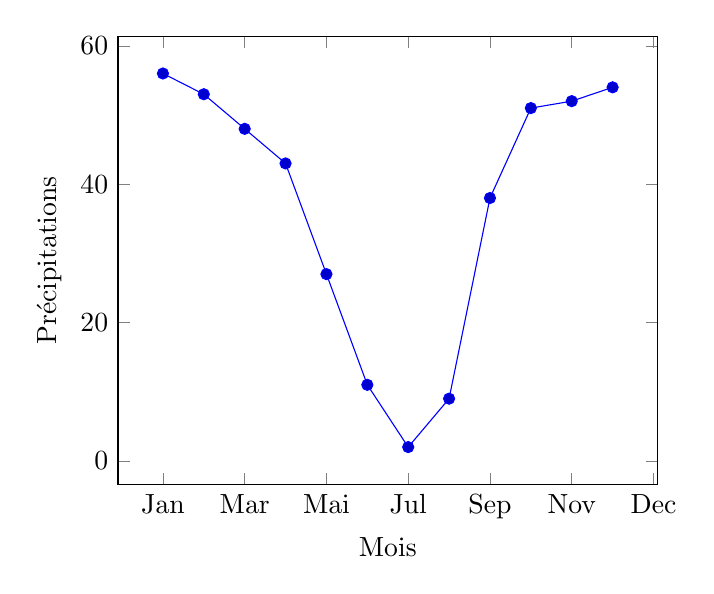
\begin{tikzpicture}
\begin{axis}[
ylabel=Précipitations,
xlabel=Mois,
symbolic x coords={Jan,Fev,Mar,Avr,Mai,Jun,Jul,Agu,
Sep,Oct,Nov,Dec},
%x tick label style={rotate=45,anchor=east}
%xtick distance=1
]
\addplot coordinates {
(Jan,56) (Fev,53) (Mar,48) (Avr,43) (Mai,27) (Jun,11) (Jul,2) (Agu,9) (Sep,38) (Oct,51) (Nov,52) (Dec,54)
};
\end{axis}
\end{tikzpicture}
\end{center}
\end{Ex}

\end{pageCours}




\begin{pageAD}

\Sf{Lire un diagramme cartésien }

\ExoCad{Chercher.}

 
\Sf{Construire un diagramme cartésien }

\ExoCad{Représenter. Calculer.}

 


\end{pageAD}



%%%%%%%%%%%%%%%%%%%%%%%%%%%%%%%%%%%%%%%%%%%%%%%%%%%%%%%%%%%%%%%%%%%
%%%  Niveau 1
%%%%%%%%%%%%%%%%%%%%%%%%%%%%%%%%%%%%%%%%%%%%%%%%%%%%%%%%%%%%%%%%%%
\begin{pageParcoursu} 

\ExoCu{Chercher. Communiquer.}

 
 
\end{pageParcoursu}


%%%%%%%%%%%%%%%%%%%%%%%%%%%%%%%%%%%%%%%%%%%%%%%%%%%%%%%%%%%%%%%%%%%
%%%%  Niveau 2
%%%%%%%%%%%%%%%%%%%%%%%%%%%%%%%%%%%%%%%%%%%%%%%%%%%%%%%%%%%%%%%%%%%
\begin{pageParcoursd} 


\ExoCd{Représenter. Calculer.} 

 
 
 
 
\end{pageParcoursd}

%%%%%%%%%%%%%%%%%%%%%%%%%%%%%%%%%%%%%%%%%%%%%%%%%%%%%%%%%%%%%%%%%%%
%%%%  Niveau 3
%%%%%%%%%%%%%%%%%%%%%%%%%%%%%%%%%%%%%%%%%%%%%%%%%%%%%%%%%%%%%%%%%%%
\begin{pageParcourst}


\ExoCt{Modéliser. Calculer.}

 
 
\end{pageParcourst}

%%%%%%%%%%%%%%%%%%%%%%%%%%%%%%%%%%%%%%%%%%%%%%%%%%%%%%%%%%%%%%%%%%%
%%%%  Brouillon
%%%%%%%%%%%%%%%%%%%%%%%%%%%%%%%%%%%%%%%%%%%%%%%%%%%%%%%%%%%%%%%%%%%


\begin{pageBrouillon} 
 
\ligne{32}



\end{pageBrouillon}



\begin{pageAuto} 

\ExoAuto
 
\ExoAuto
 



\ExoAuto

 

 



\end{pageAuto}
